
\documentclass[preprint,12pt]{elsarticle}
\makeatletter
\def\ps@pprintTitle{%
 \let\@oddhead\@empty
 \let\@evenhead\@empty
 \def\@oddfoot{\centerline{\thepage}}%
 \let\@evenfoot\@oddfoot}
\makeatother
\usepackage[spanish]{babel}
\usepackage{amssymb}
\usepackage{graphicx}
\usepackage{lineno}
\usepackage[utf8]{inputenc}
\usepackage{url}
\usepackage{natbib} 
\usepackage{amsmath} 
\usepackage{amssymb} 

\begin{document}
	\begin{frontmatter}
		\title{\huge Practica de Laboratorio Nro 09 : Instalación y Gestión de una base de datos MongoDB}
		\address{Universidad Privada de Tacna}
		\address{Escuela Profesional de Ingeniería de Sistemas}
		\address{Curso : Base de Datos II}		
		\author{Gonzales Cave, Angel Gabriel              	(2017057861)}		
		\address{Tacna, Perú}
\end{frontmatter}

%% INFORMACIÓN GENERAL -----------------------------------------------------------------------------------------------------------------------------------
\section{INFORMACIÓN GENERAL}
Objetivos:
\begin{itemize}
\item Realizar la instalacion de la Base de Datos NoSQL documental MongoDB
\item Importar un archivo JSON con colecciones de datos a MongoDB
\item Realizar consultas de registros
\end{itemize}

Requerimientos

Hardware
\begin{itemize}
\item Virtualization activada en el BIOS.
\item CPU SLAT capable feature.
\item Al menos 4GB de RAM.
\end{itemize}

Software
\begin{itemize}
\item Windows 10 64 bit
\item Docker Desktop
\end{itemize}

%% PROCEDIMIENTO -----------------------------------------------------------------------------------------------------------------------------------
\section{DESARROLLO}
\textbf{Parte I : Instalación de MongoDB}
\begin{enumerate}[a)]
\item Ingresamos a la siguiente dirección (https://www.mongodb.com/download-center/community) para descargar el instalador.
\begin{figure}[htb]
	\begin{center}
		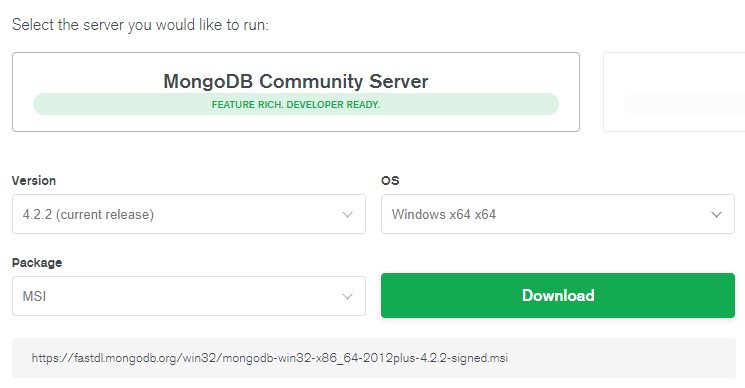
\includegraphics[width=10cm]{./IMAGENES/Mongo01}
	\end{center}
\end{figure}
\item Iniciar el instalador como administrador.
\begin{figure}[htb]
	\begin{center}
		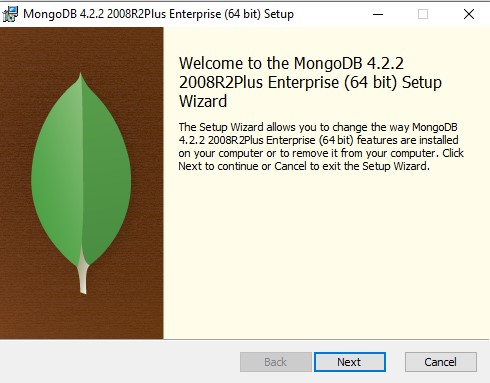
\includegraphics[width=6cm]{./IMAGENES/Mongo02}
	\end{center}
\end{figure}

\item Crear las carpetas de almacenamiento y configuración de MongoDB.
Dar permisos escritura y lectura a estas carpetas.
C:/data - C:/data/db
\begin{figure}[htb]
	\begin{center}
		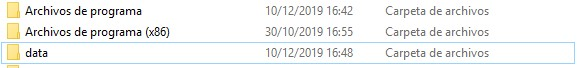
\includegraphics[width=10cm]{./IMAGENES/Mongo03}
	\end{center}
\end{figure}

\item Iniciar el servidor del servicio de MongoDB: mongod. Primero dirigir a la siguiente ruta (C:/Program Files/MongoDB/Server/4.2/bin). Y ejecutar el comando mongod:
\begin{figure}[htb]
	\begin{center}
		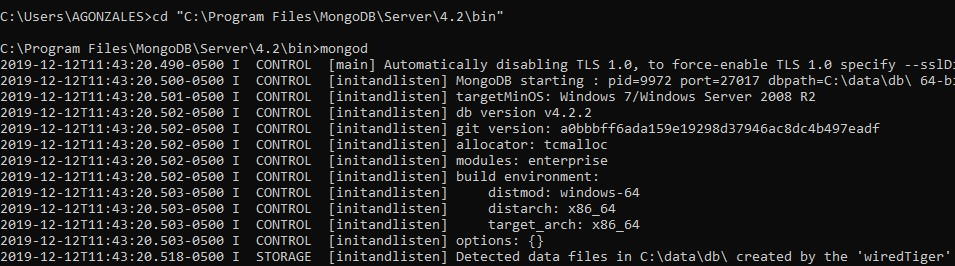
\includegraphics[width=13cm]{./IMAGENES/Mongo04}
	\end{center}
\end{figure}

\item Iniciar el shell de mongo : mongo.exe
\begin{figure}[htb]
	\begin{center}
		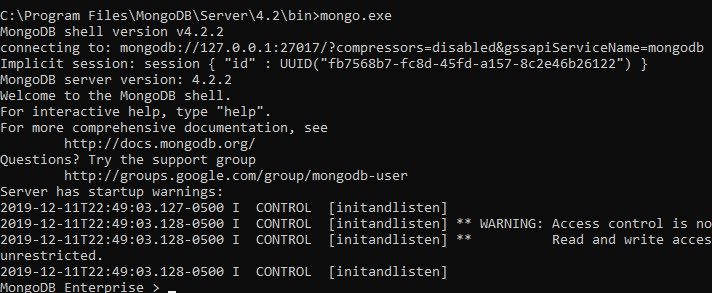
\includegraphics[width=13cm]{./IMAGENES/Mongo05}
	\end{center}
\end{figure}

\textbf{Parte II: Importar Datos}
\item Para importar datos utilizaremos el comandoimport. Este comando es capaz de importar datos en distintos formatos a nuestra base de datos.\newline 
(mongoimport.exe --host localhost --port 27017 --db test --collection people --type json --file C:/Users/AGONZALES/Documents/mongodb-consultas.json)
\begin{figure}[htb]
	\begin{center}
		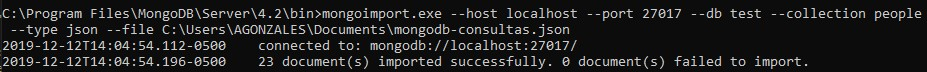
\includegraphics[width=13cm]{./IMAGENES/Mongo07}
	\end{center}
\end{figure}

\item Con este comando, lo que haremos será incorporar los datos a nuestro servidor, que está en el puerto 27017, concretamente a una base de datos llamada test y a una colección que hemos llamado people.\newline

\textbf{Parte III : Consultas}
\item Iniciar el shell de mongo mongo.exe. \newline
\begin{figure}[htb]
	\begin{center}
		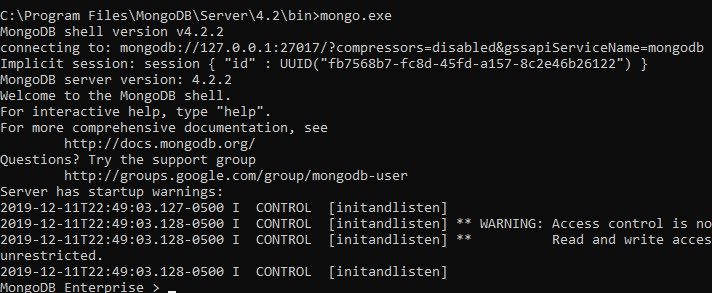
\includegraphics[width=13cm]{./IMAGENES/Mongo05}
	\end{center}
\end{figure}

\item Para realizar consultas a la base de datos, deberemos usar el comando db.nombredecoleccion.find(). Este comando puede recibir dos parámetros: una consulta y una proyección. Ambos comandos son opcionales por lo que si ejecutamos el comando: 'db.people.find()'.
\begin{figure}[htb]
	\begin{center}
		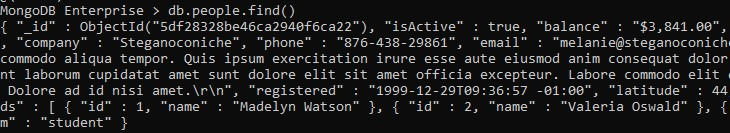
\includegraphics[width=13cm]{./IMAGENES/Mongo08}
	\end{center}
\end{figure}
\newline

\item Obtendremos una larga lista con los 20 elementos de la colección. Al ejecutar el comando podemos ver que el resultado no está demasiado formateado, por lo que es muy difícil leerlo. Para solucionar este problema podemos usar el modificador pretty que nos devolverá un resultado mucho más legible 'db.people.find().pretty()'.

\begin{figure}[htb]
	\begin{center}
		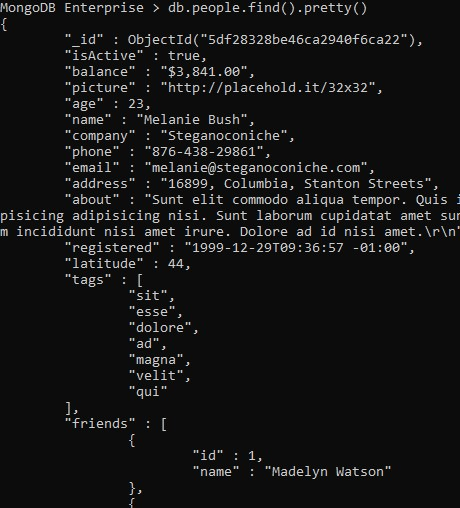
\includegraphics[width=8.5cm]{./IMAGENES/Mongo09}
	\end{center}
\end{figure}

\item Ahora vamos a añadir la consulta al comando find, para que filtre los elementos según nuestras necesidades. Para ello especificaremos un objeto JSON como primer parámetro del comando, con los campos por los que queremos filtrar:

db.people.find(
{age:34}
).pretty()

\begin{figure}[htb]
	\begin{center}
		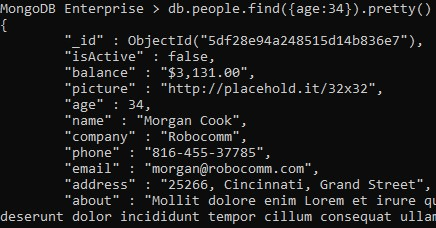
\includegraphics[width=7.8cm]{./IMAGENES/Mongo010}
	\end{center}
\end{figure}

\item Con ese comando obtendremos las personas cuya edad es de 34 años. Podemos añadir tantos filtros como queramos.

db.people.find(
{age:34,isActive:true}
).pretty()

\begin{figure}[htb]
	\begin{center}
		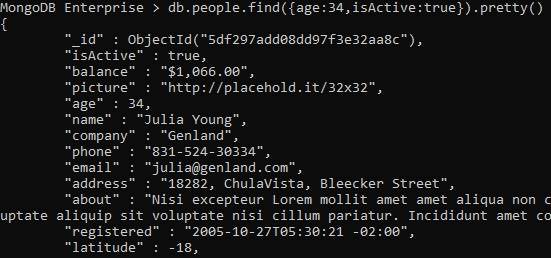
\includegraphics[width=10cm]{./IMAGENES/Mongo011}
	\end{center}
\end{figure}

\item En este caso filtramos por age y por isActive. Como se ve los resultados nos muestran todos los campos de cada elemento. Es como si hubiésemos utilizado el asterisco en una consulta SELECT. Si queremos solo algunos de los campos, deberemos utilizar el segundo parámetro de la consulta find para definir una proyeccion.

db.people.find(
{age:34,isActive:true},
{name:1,age:1,isActive:1}
).pretty()

\begin{figure}[htb]
	\begin{center}
		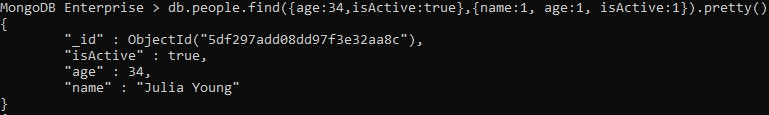
\includegraphics[width=13cm]{./IMAGENES/Mongo012}
	\end{center}
\end{figure}

\item Que no devuelve solo los campos que se requieren, además del id. El id por defecto se muestra siempre, así que si queremos ocultarlo hay que especificarlo en la proyección.

db.people.find(
{age:34,isActive:true},
{name:1,age:1,isActive:1,id:0}

\begin{figure}[htb]
	\begin{center}
		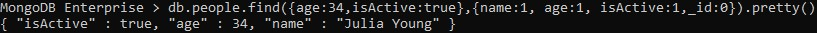
\includegraphics[width=13cm]{./IMAGENES/Mongo013}
	\end{center}
\end{figure}

\item Si queremos mostrar todos los campos, pero quitando solo algunos, lo que haremos será desactivar los no deseados en la proyección:

db.people.find(\newline
{age:34,isActive:true},\newline
{name:0,age:0,isActive:0,id:0}).pretty()\newline

\begin{figure}[htb]
	\begin{center}
		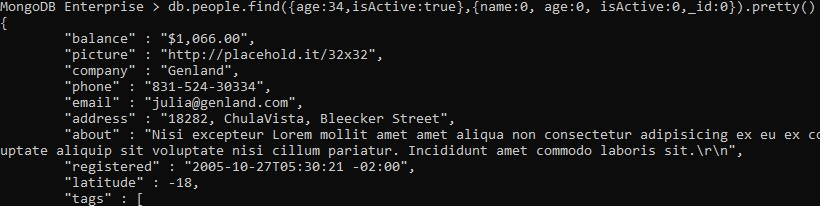
\includegraphics[width=13cm]{./IMAGENES/Mongo014}
	\end{center}
\end{figure}

\item El comando findOne tiene el mismo funcionamiento que el comando find, con la diferencia de que, si el comando encuentra más de un resultado que cumpla las condiciones de la consulta, tan solo nos devolverá el primero.

db.people.findOne({age:34,isActive:true},{name:0,age:0,isActive:0,id:0})

\begin{figure}[htb]
	\begin{center}
		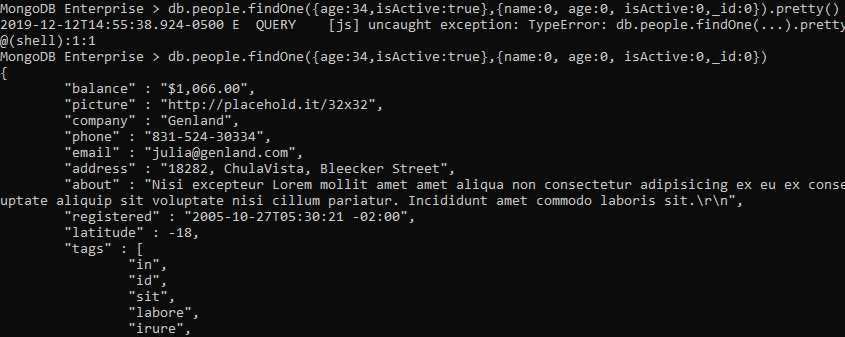
\includegraphics[width=13cm]{./IMAGENES/Mongo015}
	\end{center}
\end{figure}

\item Además findOne no acepta pretty, pero ya devuelve el resultado formateado.

\begin{figure}[htb]
	\begin{center}
		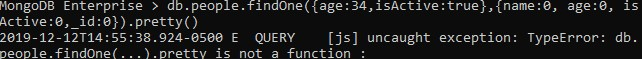
\includegraphics[width=13cm]{./IMAGENES/Mongo016}
	\end{center}
\end{figure}

\item En las consultas, en cambio, no se ha especificado dichas comillas. Esto es porque el motor JavaScript de MongoDB se encarga de añadirlas. Esto nos facilita la escritura de consultas, ya que no son obligatorias. De hecho, la siguiente consulta, funcionará perfectamente:

db.people.findOne(\newline
{“age”:34,”isActive”:true},\newline
{“name”:0,”age”:0,”isActive”:0,”id”:0})\newline

\begin{figure}[htb]
	\begin{center}
		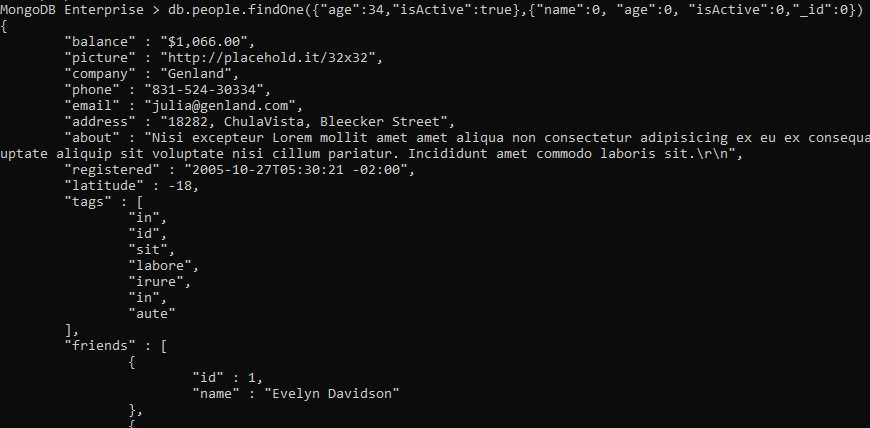
\includegraphics[width=15cm]{./IMAGENES/Mongo017}
	\end{center}
\end{figure}

\end{enumerate}
\end{document}
